\section{Experiment}

We evaluate \textbf{MP-Init} and \textbf{TrSG} on both static and event-based vision benchmarks, including CIFAR10, CIFAR100~\cite{cifar}, ImageNet~\cite{imagenet}, and DVS-CIFAR10~\cite{dvscifar10}, using diverse backbones such as ResNet-19~\cite{zheng:2021}, a 7-layer CNN~\cite{tebn:2022,tab:2024}, ResNet-34~\cite{resnet}, and SEW-ResNet-34~\cite{fang:2021_2}. Following tdBN~\cite{zheng:2021}, batch normalization is applied across both temporal and batch dimensions. All baselines are trained under their original configurations, and we strictly follow their reported preprocessing pipelines for fairness. We avoid strong augmentations such as AutoAugment~\cite{autoaug} or Cutout~\cite{cutout} to ensure that observed gains come solely from our proposed methods. We run three independent trials and report the results as \(\mathbf{mean}\pm\mathbf{std}\) across runs. Detailed descriptions of architectures, preprocessing, and hyperparameters are provided in the supplementary material (\cref{sec:experimental_detail}).



\begin{table}[t]
\small
\centering
\begin{tabular}{cccc}
\toprule
\textbf{Dataset}     & \textbf{Method}    & \textbf{Timestep} & \textbf{Accuracy (\%)} \\
\toprule
\multirow{6}{*}{CIFAR100}    & tdBN      & \multirow{2}{*}{4} & 75.55 ± 0.06 \\ 
                             & + MP-Init &                    & \textbf{76.09 ± 0.04}    \\
\cline{2-4}
                             & TEBN      & \multirow{2}{*}{4} & 75.96 ± 0.68    \\
                             & + MP-Init &                    & \textbf{76.45 ± 0.24}    \\
\cline{2-4}
                             & TAB       & \multirow{2}{*}{4} & 76.25 ± 0.49    \\
                             & + MP-Init &                    & \textbf{77.24 ± 0.12}    \\ 
\hlineB{1.5}
\multirow{6}{*}{DVS-CIFAR10} & tdBN      & \multirow{2}{*}{10} & 76.60 ± 0.20    \\
                             & + MP-Init &                     & \textbf{77.37 ± 0.38}    \\
\cline{2-4}
                             & TEBN      & \multirow{2}{*}{10} & 75.17 ± 0.50    \\
                             & + MP-Init &                     & \textbf{76.70 ± 0.78}    \\
\cline{2-4}
                             & TAB       & \multirow{2}{*}{4} & 76.43 ± 0.25    \\
                             & + MP-Init &                     & \textbf{76.93 ± 0.38}    \\ 
\bottomrule
\end{tabular}
\vspace{-0.5em}
\caption{Validation of performance improvements from MP-Init using ResNet-19 on CIFAR100 and DVS-CIFAR10 datasets.}
\label{tab:mpinit_acc_impr}
\end{table}


\begin{figure}[t]
  \centering
  \begin{subfigure}{0.32\linewidth}
    \centering
    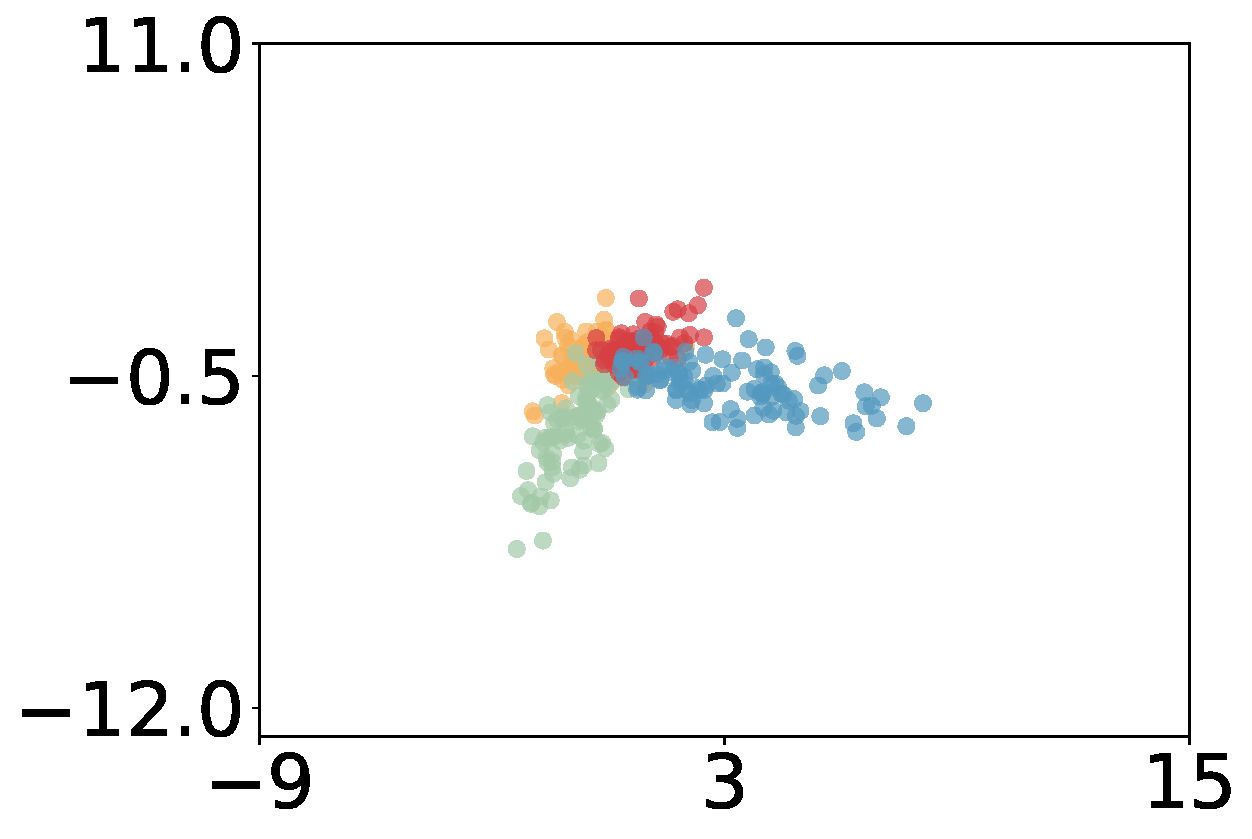
\includegraphics[width=0.995\linewidth]{fig/feature_map_not_mp_init_0.pdf}
    \caption{t = 1}
  \end{subfigure}
  \begin{subfigure}{0.32\linewidth}
    \centering
    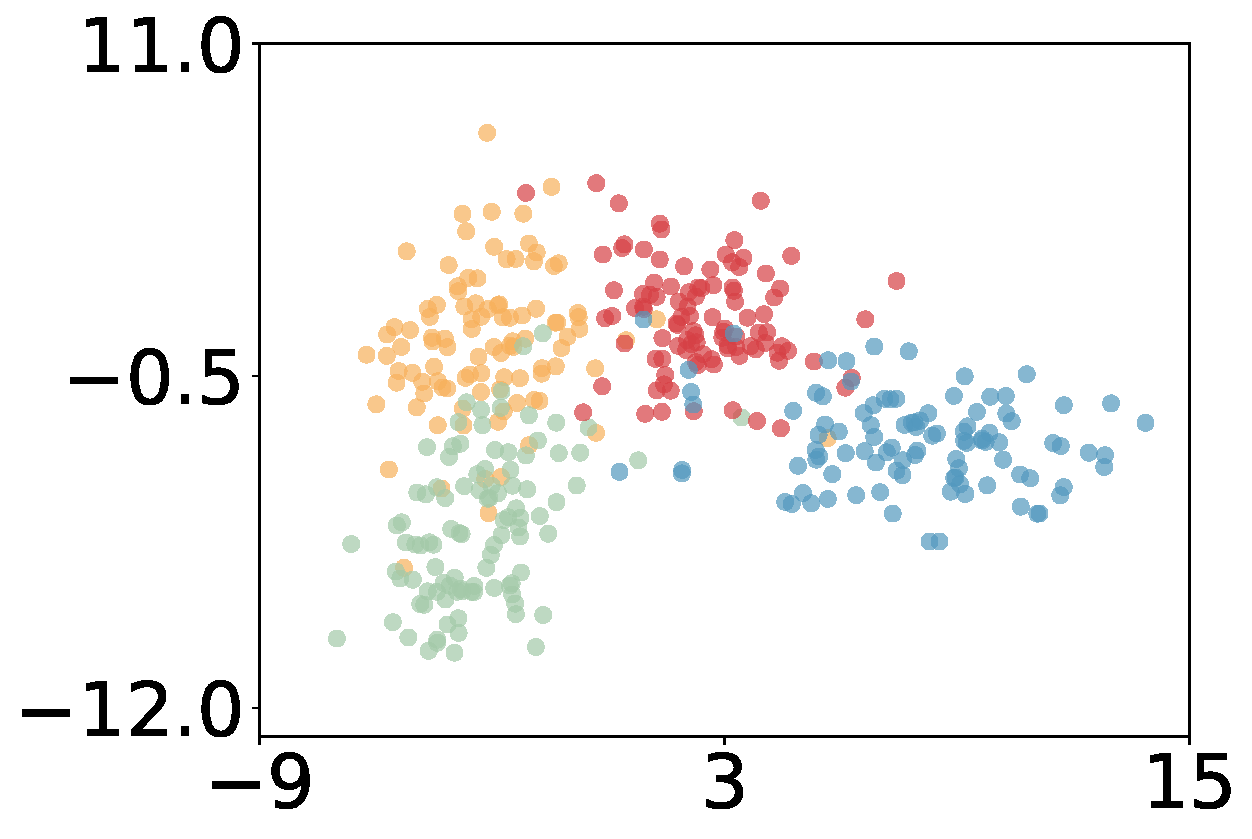
\includegraphics[width=0.995\linewidth]{fig/feature_map_not_mp_init_1.pdf}
    \caption{t = 2}
  \end{subfigure}
  \begin{subfigure}{0.32\linewidth}
    \centering
    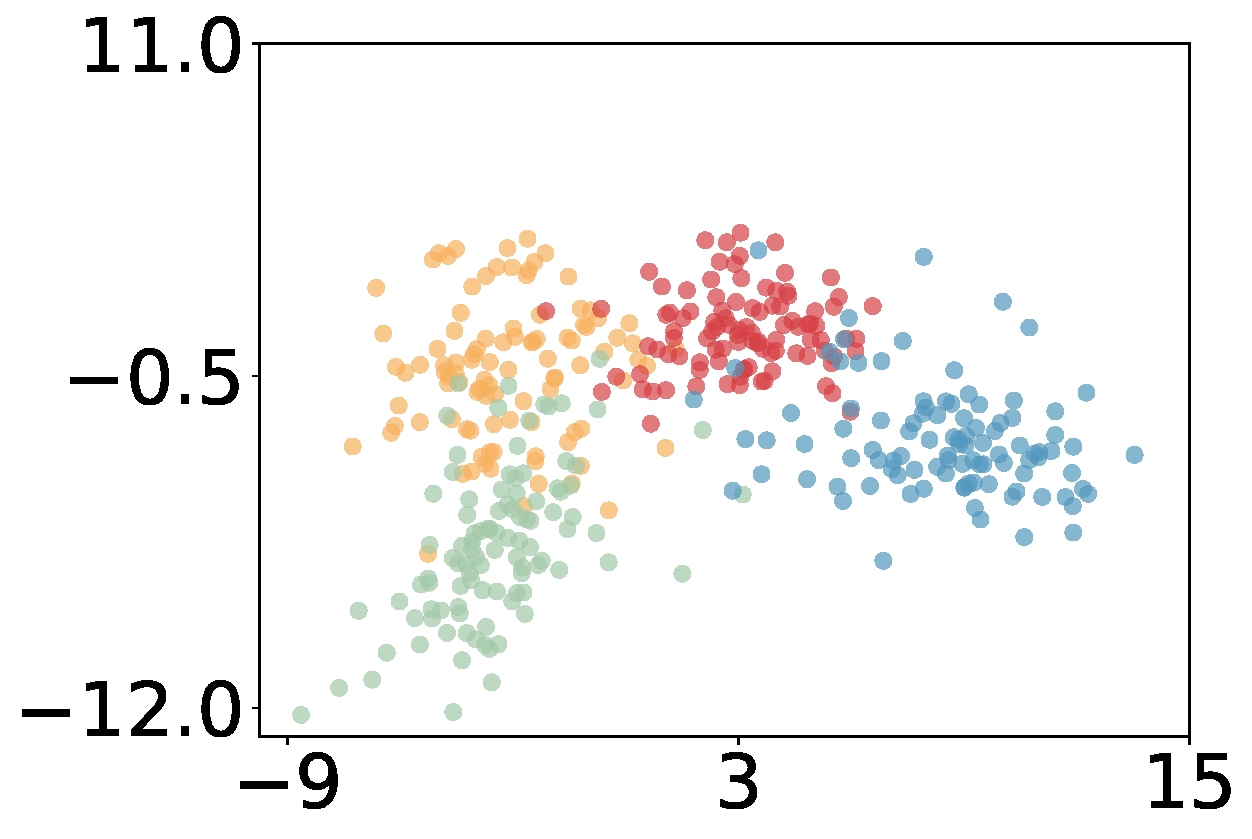
\includegraphics[width=0.995\linewidth]{fig/feature_map_not_mp_init_3.pdf}
    \caption{t = 4}
  \end{subfigure}
  \vspace{-0.5em}
  \caption{PCA of logits without MP-Init. Class clusters stay mixed in early timesteps, showing strong temporal covariate shift.}
  \label{fig:feature_split_wo_mpinit}
\end{figure}

\begin{figure}[t]
  \centering
  \begin{subfigure}{0.32\linewidth}
    \centering
    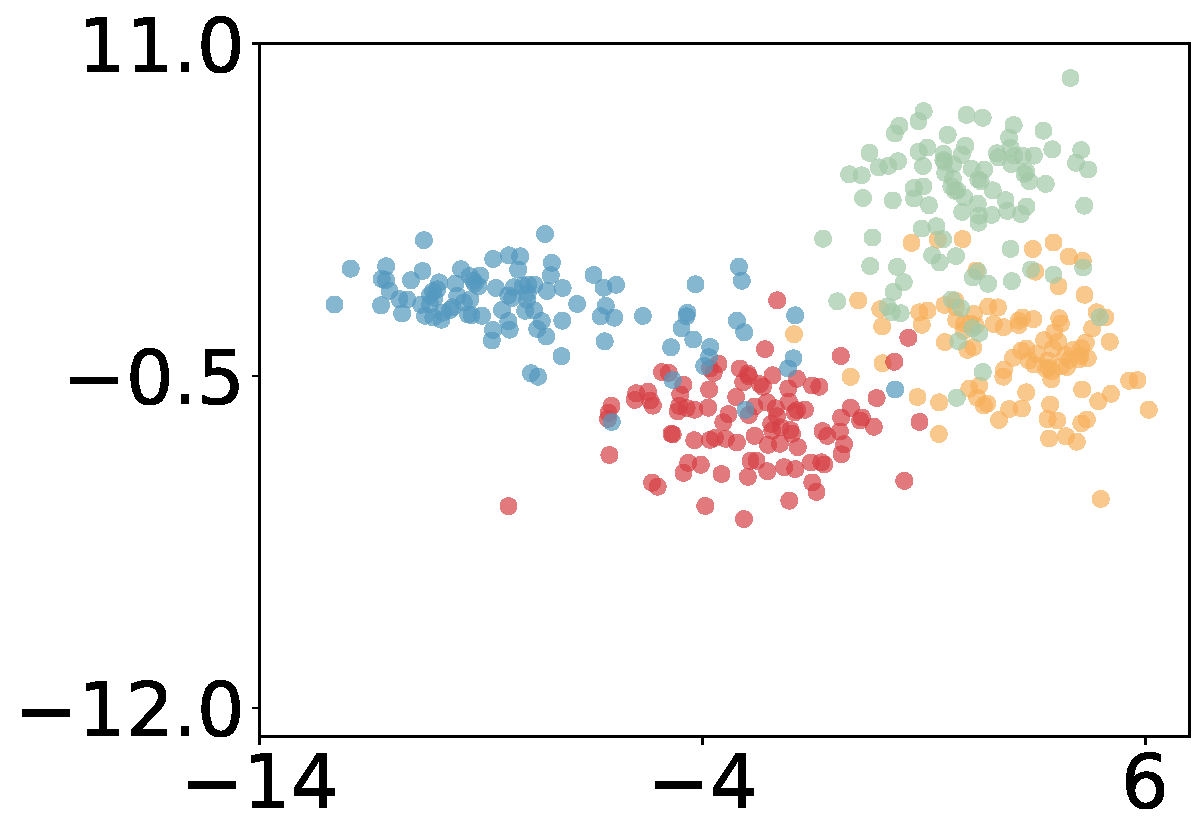
\includegraphics[width=0.995\linewidth]{fig/feature_map_mp_init_0.pdf}
    \caption{t = 1}
  \end{subfigure}
  \begin{subfigure}{0.32\linewidth}
    \centering
    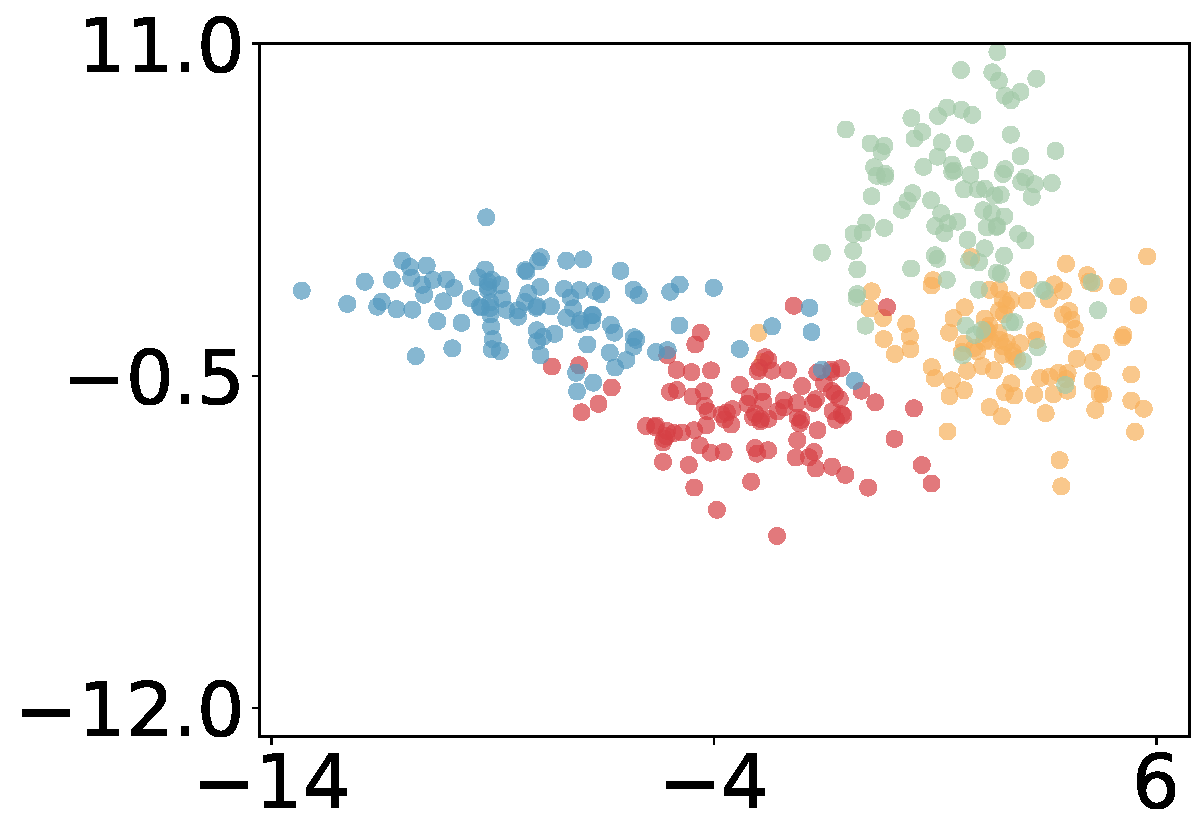
\includegraphics[width=0.995\linewidth]{fig/feature_map_mp_init_1.pdf}
    \caption{t = 2}
  \end{subfigure}
  \begin{subfigure}{0.32\linewidth}
    \centering
    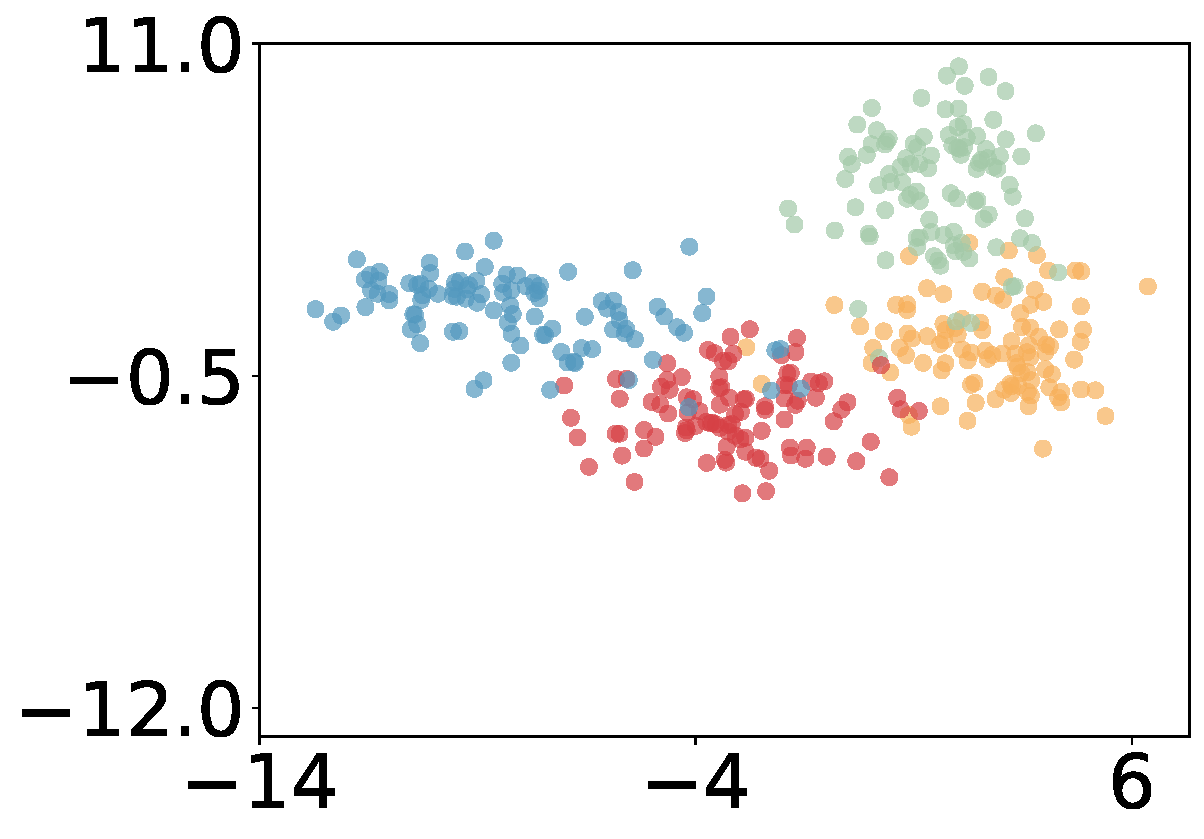
\includegraphics[width=0.995\linewidth]{fig/feature_map_mp_init_3.pdf}
    \caption{t = 4}
  \end{subfigure}
  \vspace{-0.5em}
  \caption{PCA of logits with MP-Init. Clear class separation emerges from t=1, indicating reduced temporal drift.}
  \label{fig:feature_split_w_mpinit}
\end{figure}

\subsection{Analysis of MP-Init}
\label{subsec:analysis_of_mpinit}

\paragraph{Effectiveness of MP-Init}

We begin by assessing whether MP-Init effectively enhances the final performance of SNNs. To do this, we train ResNet-19 on CIFAR100 and DVS-CIFAR10 datasets and measure accuracy with and without MP-Init, as shown in Table~\ref{tab:mpinit_acc_impr}. We observe consistent performance improvements with MP-Init, not only in tdBN, which does not account for TCS, but also in TCS-aware methods such as TEBN and TAB. This consistency suggests that previous approaches may only partially address the TCS issue, whereas MP-Init offers a more fundamental solution. Additional analysis on how MP-Init affects training is provided in \cref{subsec:how_mpinit}.

\begin{figure}[t]
  \centering
  \begin{subfigure}{0.49\linewidth}
    \centering
    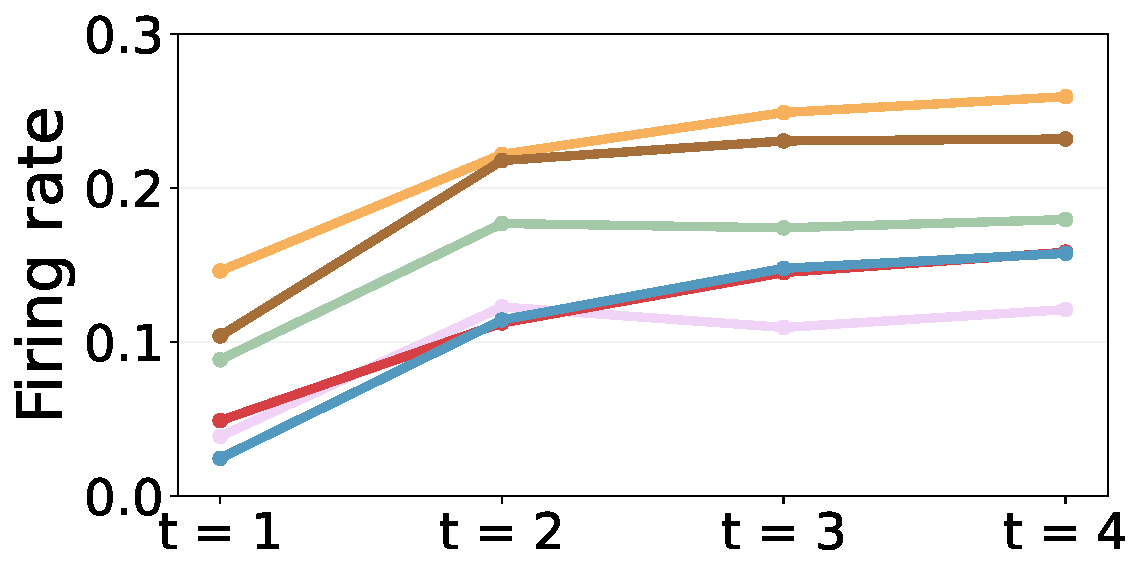
\includegraphics[width=0.99\linewidth]{fig/firing_rate_not_mp_init.pdf}
    \caption{w/o MP-Init}
  \end{subfigure}
  \hfill
  \begin{subfigure}{0.49\linewidth}
    \centering
    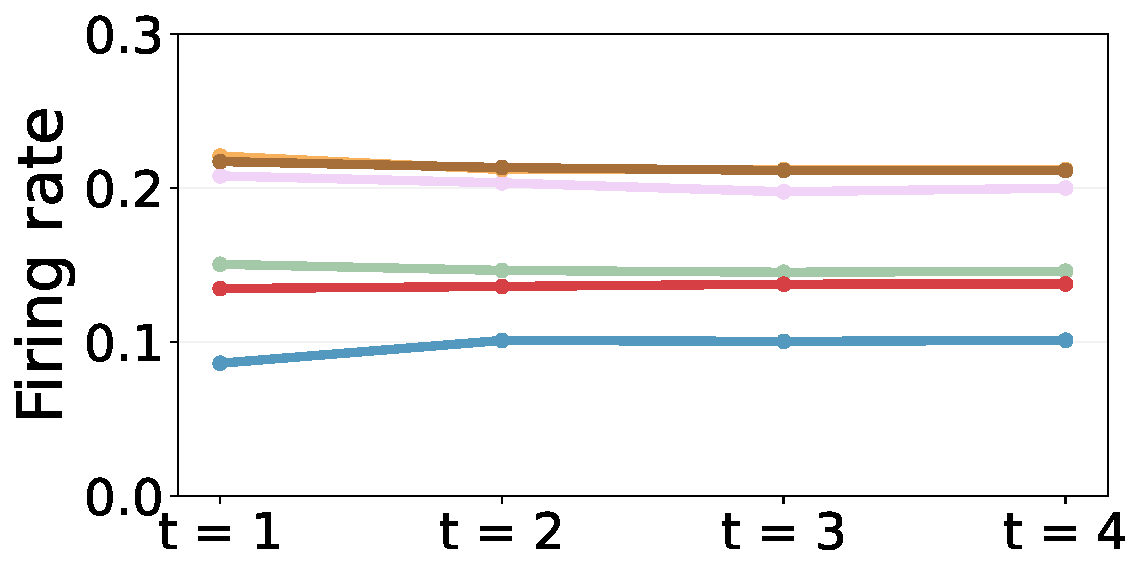
\includegraphics[width=0.99\linewidth]{fig/firing_rate_mp_init.pdf}
    \caption{w/ MP-Init}
  \end{subfigure}
  \vspace{-0.5em}
  \caption{Firing rate of all neurons at each timestep in arbitrarily selected 6 layers of ResNet-19 on CIFAR10.}
  \label{fig:firing_rate_at_timestep}
\end{figure}

\begin{figure}[t!]
  \centering
  \begin{subfigure}{0.49\linewidth}
    \centering
    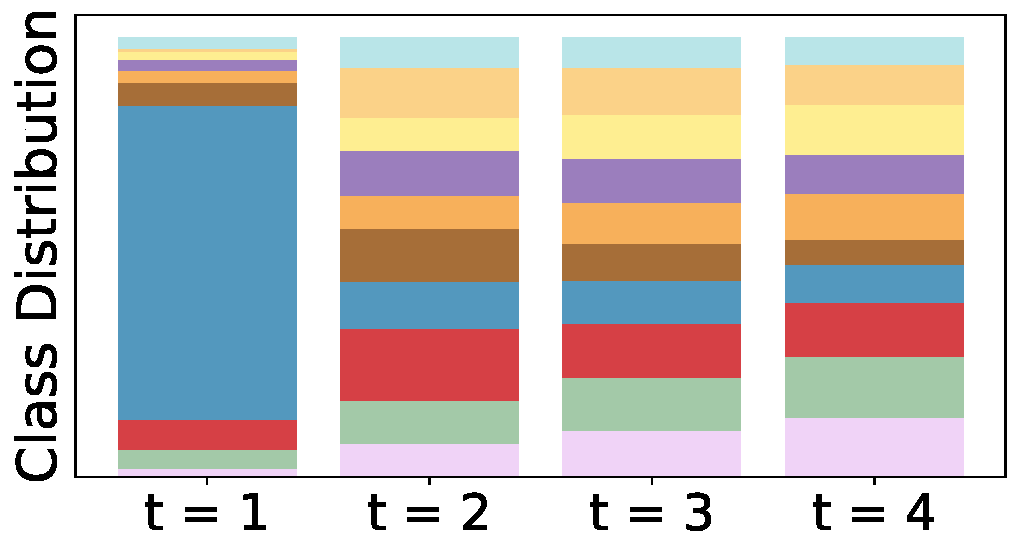
\includegraphics[width=0.99\linewidth]{fig/not_mp_init_output_rate.pdf}
    \caption{w/o MP-init}
  \end{subfigure}
  \hfill
  \begin{subfigure}{0.49\linewidth}
    \centering
    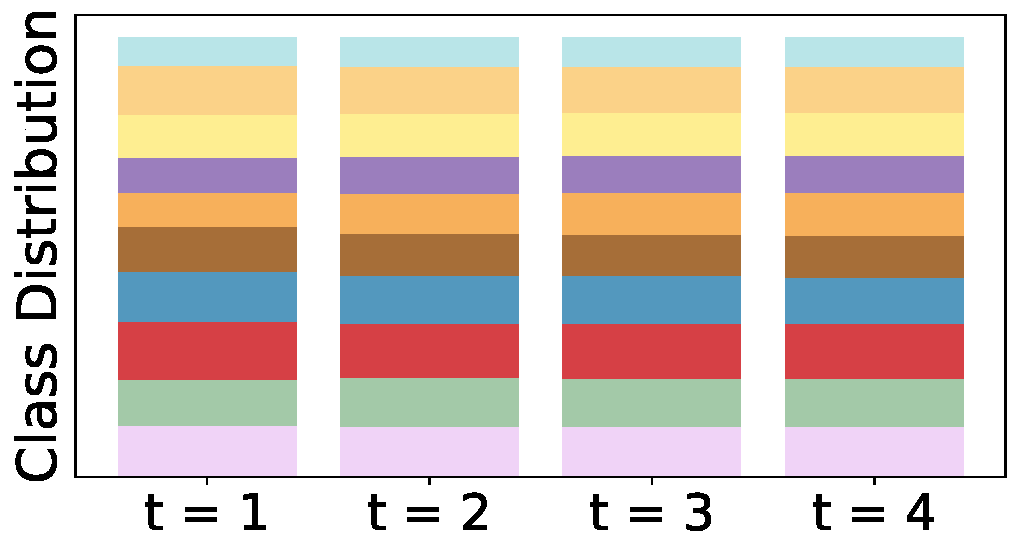
\includegraphics[width=0.99\linewidth]{fig/mp_init_output_rate.pdf}
    \caption{w/ MP-init}
  \end{subfigure}
  \vspace{-0.5em}
  \caption{Class prediction distributions over timesteps in ResNet-19 on CIFAR10. Without MP-Init, early steps collapse to a few classes; MP-Init yields balanced outputs from t=1.}
  \label{fig:classification}
\end{figure}

\begin{figure}[t]
  \centering
  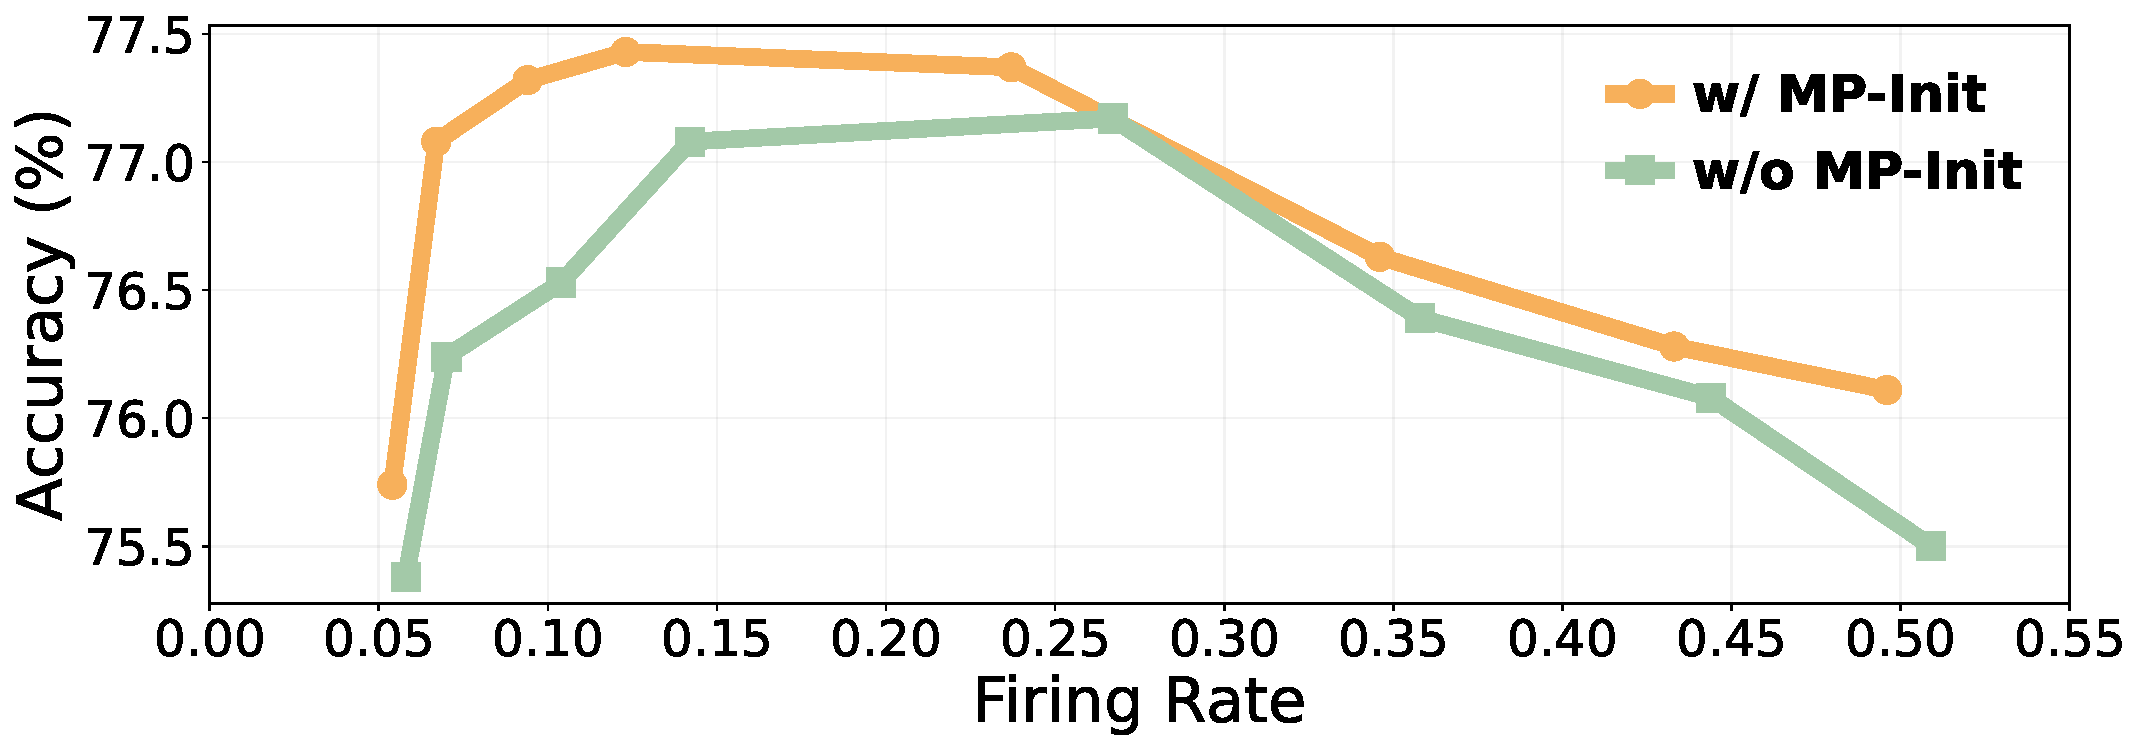
\includegraphics[width=0.98\linewidth]{fig/firing_rate_vs_accuracy.pdf}
  \vspace{-0.5em}
  \caption{Accuracy vs. firing rate. MP-Init consistently achieves higher accuracy at matched sparsity levels, forming a better Pareto frontier.}
  \label{fig:firing_rate_vs_accuracy_mpinit}
\end{figure}

\begin{figure*}[t]
    \centering
    
    %--- Top row ---%
    \begin{subfigure}[b]{0.48\textwidth}
        \centering
        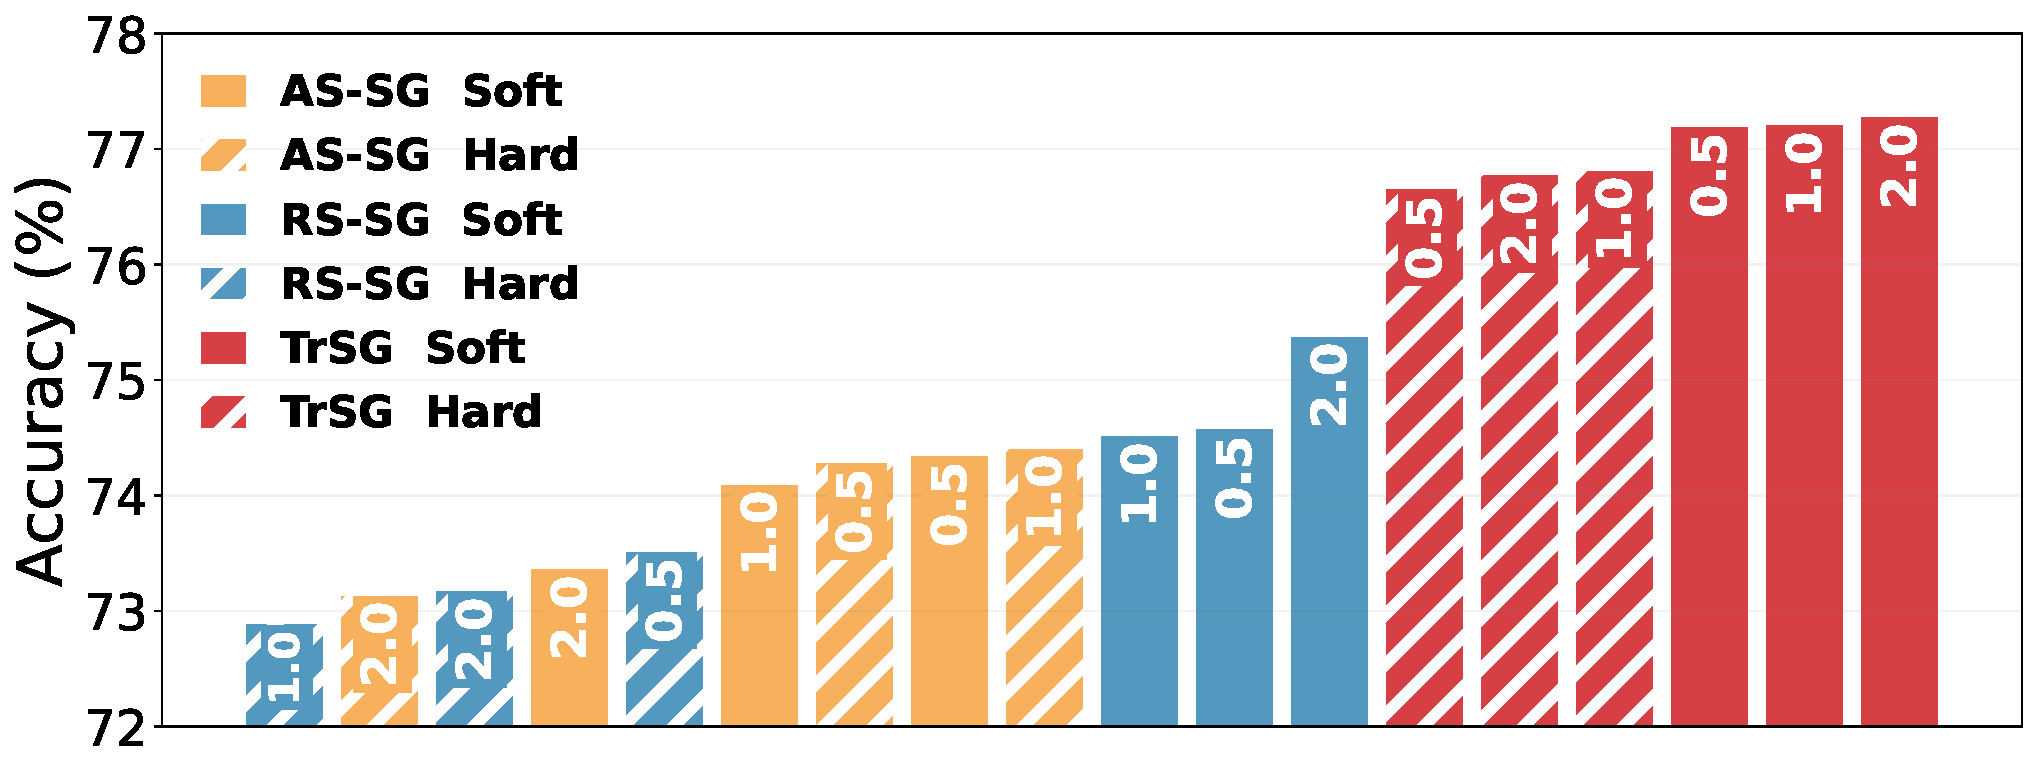
\includegraphics[width=\linewidth]{fig/acc_different_thr_rect.pdf}
        \caption{Rectangular-Shaped Surrogate Gradient}
        \label{fig:acc_rect}
    \end{subfigure}
    \hfill
    \begin{subfigure}[b]{0.48\textwidth}
        \centering
        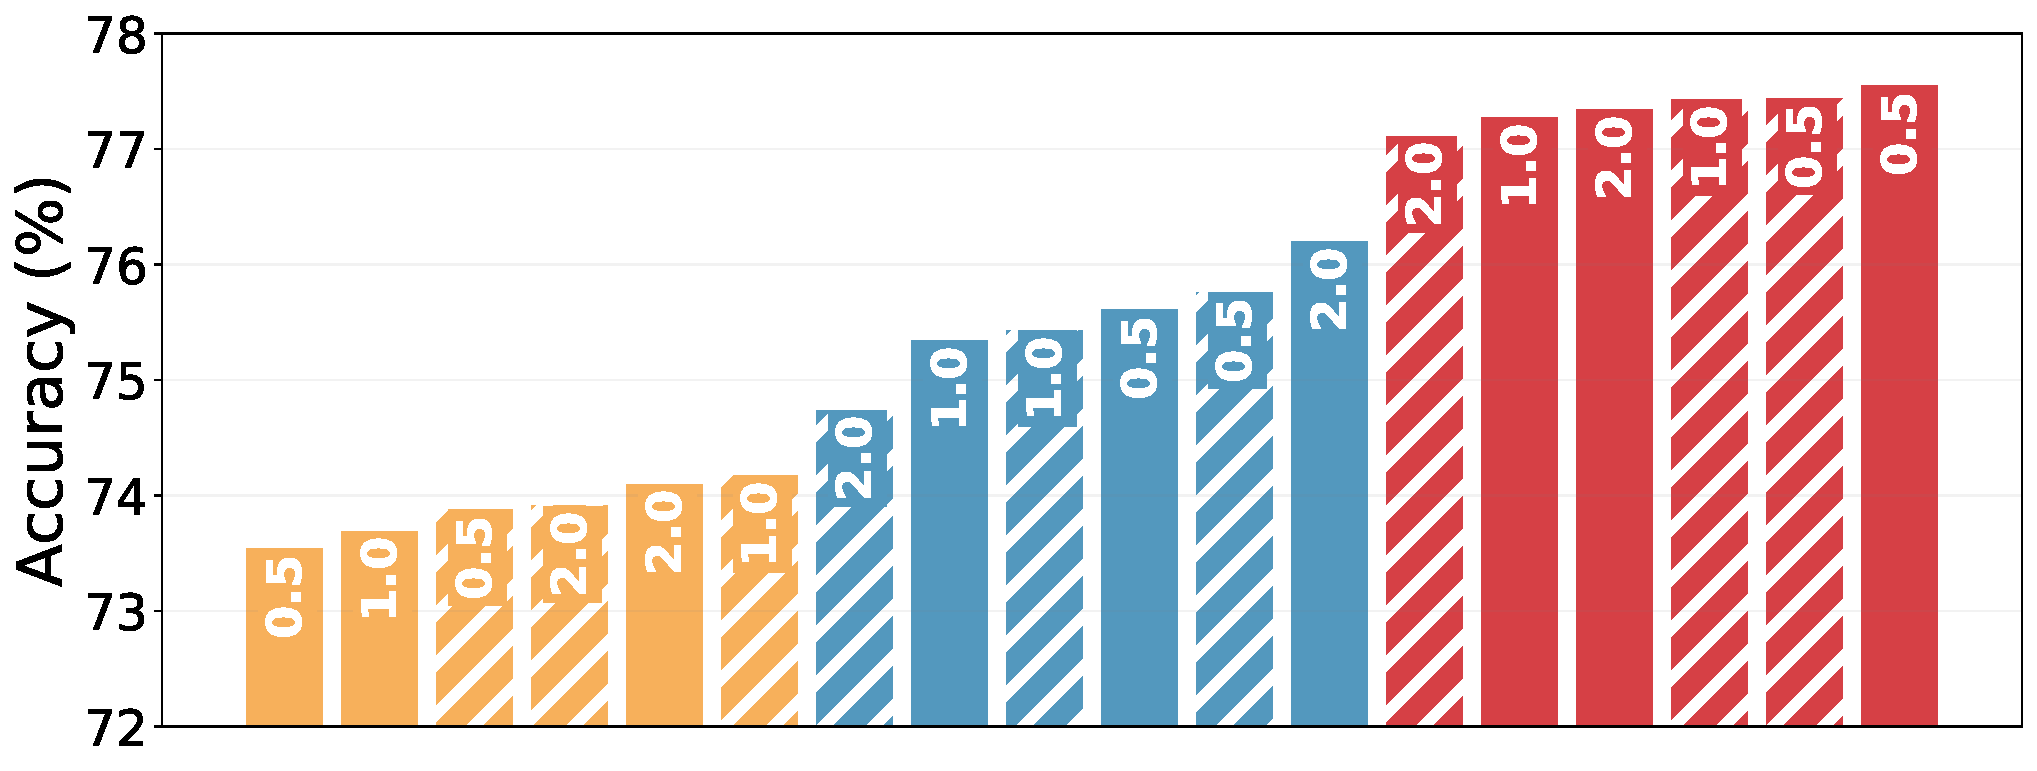
\includegraphics[width=\linewidth]{fig/acc_different_thr_tri.pdf}
        \caption{Triangular-Shaped Surrogate Gradient}
        \label{fig:acc_tri}
    \end{subfigure}
    
    % \vspace{0.5em}

    %--- Bottom row ---%
    \begin{subfigure}[b]{0.24\textwidth}
        \centering
        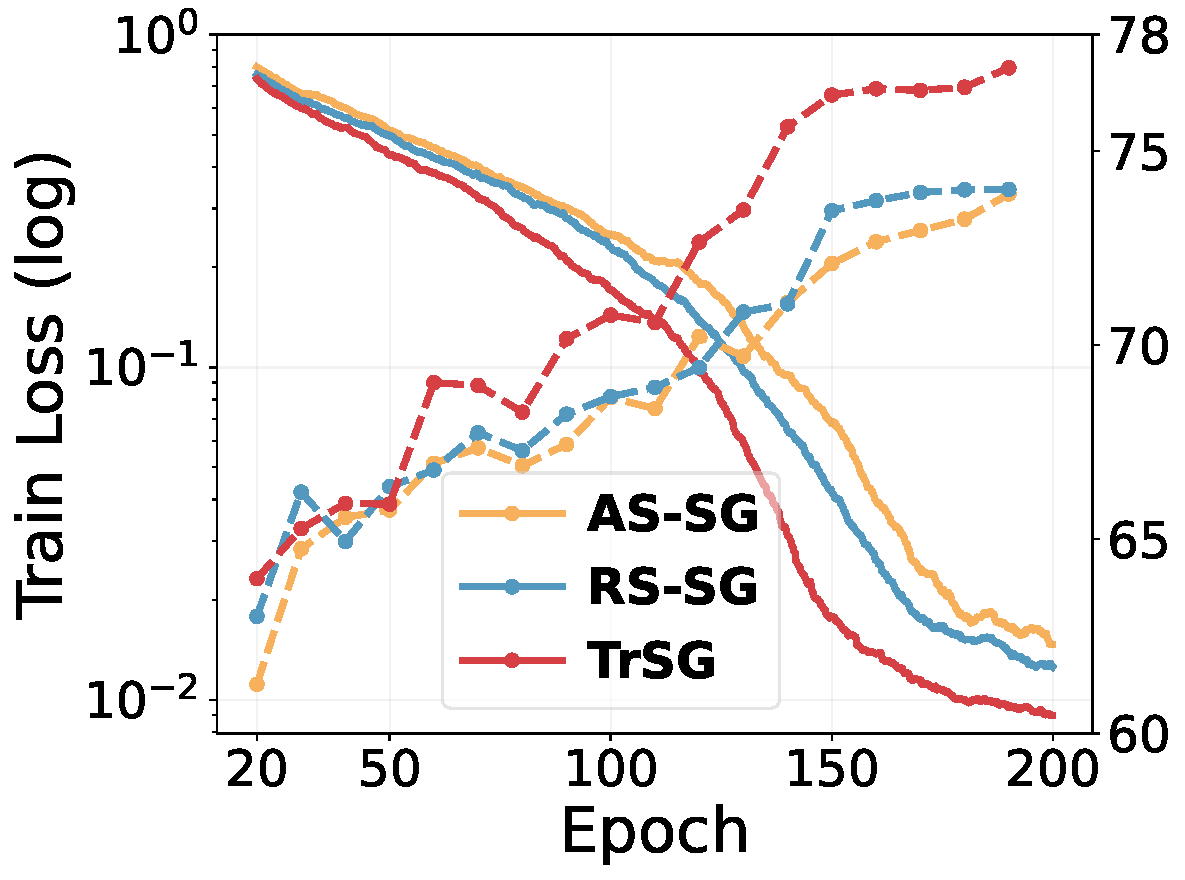
\includegraphics[width=\linewidth]{fig/loss_acc_rect_soft.pdf}
        \caption{Rectangular (soft)}
        \label{fig:rect_soft}
    \end{subfigure}
    \begin{subfigure}[b]{0.24\textwidth}
        \centering
        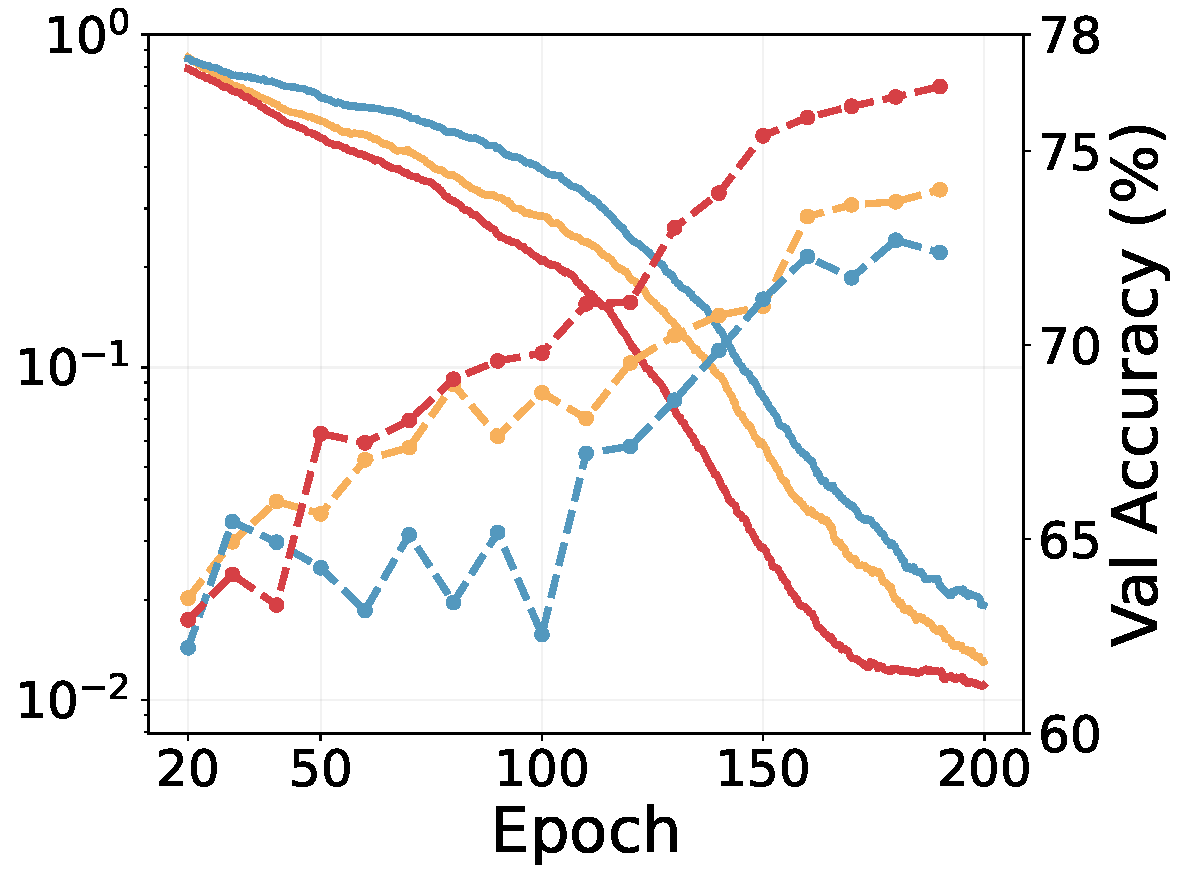
\includegraphics[width=\linewidth]{fig/loss_acc_rect_hard.pdf}
        \caption{Rectangular (hard)}
        \label{fig:rect_hard}
    \end{subfigure}
    \hfill
    \begin{subfigure}[b]{0.24\textwidth}
        \centering
        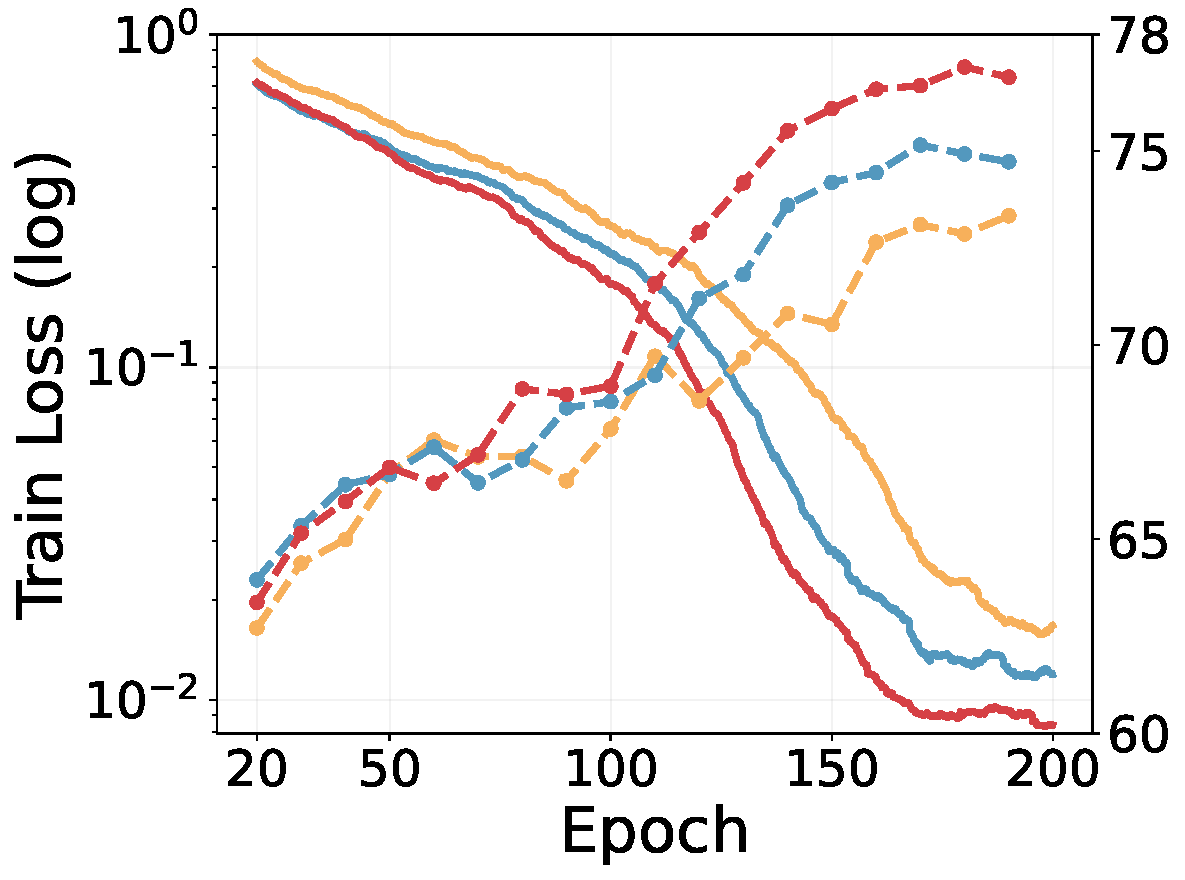
\includegraphics[width=\linewidth]{fig/loss_acc_tri_soft.pdf}
        \caption{Triangular (soft)}
        \label{fig:tri_soft}
    \end{subfigure}
    \begin{subfigure}[b]{0.24\textwidth}
        \centering
        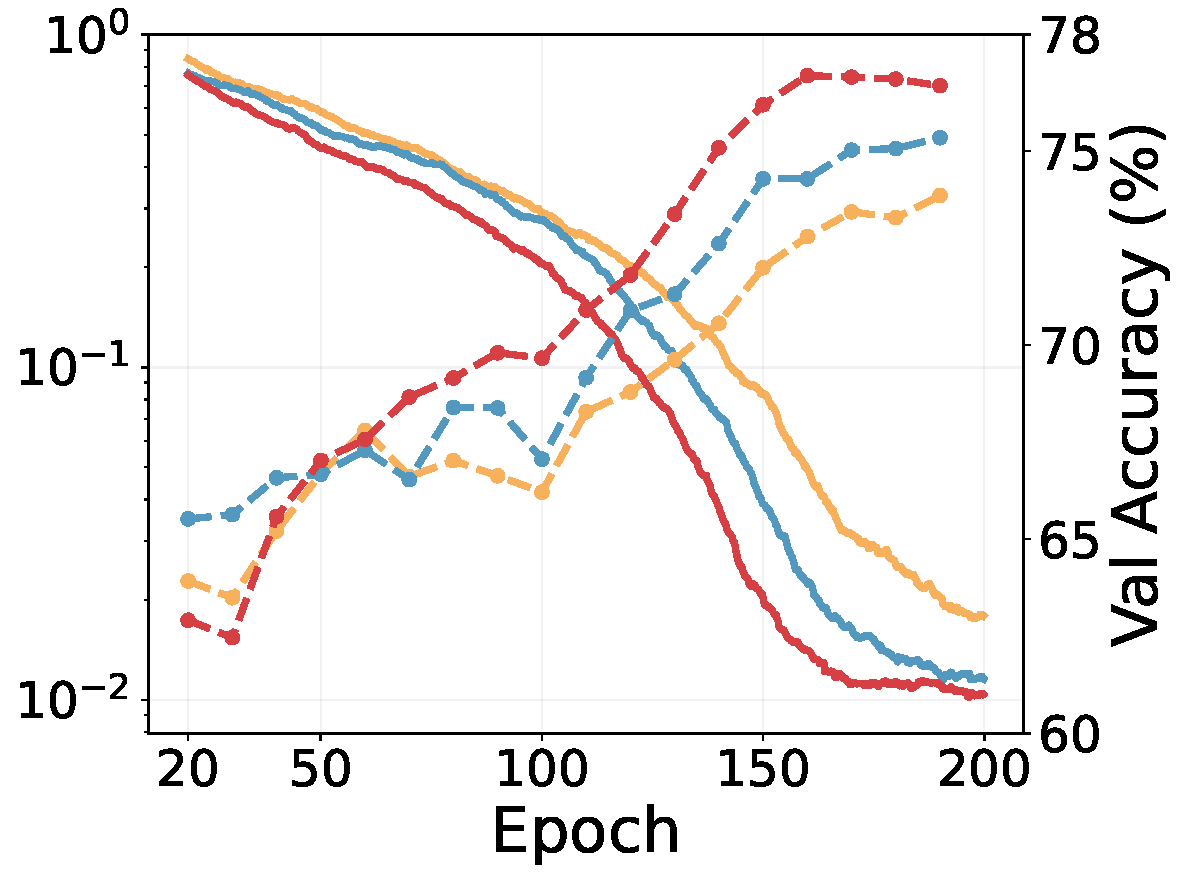
\includegraphics[width=\linewidth]{fig/loss_acc_tri_hard.pdf}
        \caption{Triangular (hard)}
        \label{fig:tri_hard}
    \end{subfigure}
    \vspace{-5pt}
    \caption{
        \textbf{Comparison of SG approaches under different surrogate function shapes (rectangular and triangular), reset types (soft and hard).}
        \textbf{(Top Row)} shows final accuracy on CIFAR100 (ResNet-19, timestep = 4) 
         at various initial $V_{\text{thr}}\in\{0.5,1.0,2.0\}$ and an initial $\tau=2.0$. 
        \textbf{(Bottom Row)} plots the training loss and validation accuracy curves with initial $\tau=2.0$ and $V_{\text{thr}}=1.0$. 
        In all experiments, \textbf{TrSG} consistently outperforms the AS-SG and RS-SG methods, demonstrating robustness to different initial values.
    }
    \label{fig:unified_fig}
    \vspace{-1em}
\end{figure*}

\paragraph{Impact of TCS and Role of MP-Init}

To visualize TCS effects, we train ResNet-19 on CIFAR10 and project the final logits of four randomly selected classes onto two principal components (\cref{fig:feature_split_wo_mpinit,fig:feature_split_w_mpinit}). Without MP-Init, these classes remain entangled in early steps and only gradually separate, reflecting TCS-induced output bias. With MP-Init, class separation emerges from the first timestep. This aligns with the firing-rate dynamics in~\cref{fig:firing_rate_at_timestep}: MP-Init stabilizes neuron activations across timesteps, whereas the baseline accumulates activity over time. Class-distribution analysis (\cref{fig:classification}) further confirms this: networks without MP-Init produce heavily skewed class predictions at early timesteps, often collapsing to a single dominant class. This illustrates the impact of temporal covariate shift on output stability. In contrast, MP-Init yields balanced class distributions from the first timestep, confirming that it mitigates early-step bias and enables reliable low-latency inference.

\paragraph{Firing Rate vs. Accuracy}
A natural concern after \cref{fig:firing_rate_at_timestep} is whether MP-Init simply increases firing and thereby harms efficiency. To test this, we apply a regularization loss~\cite{yan:2022} for ResNet-19 on CIFAR100 that directly controls spike sparsity and evaluate performance across a wide range of firing rates (\cref{fig:firing_rate_vs_accuracy_mpinit}). The results show that MP-Init does not rely on excessive spiking: it consistently forms a Pareto frontier, achieving higher accuracy than the baseline at the same or even lower firing rates. Remarkably, at a firing rate as low as 0.06, MP-Init still outperforms all baseline settings. This indicates that MP-Init not only enhances accuracy but also enables more energy-efficient SNN operation.


\subsection{Analysis of TrSG}
\label{subsec:analysis_of_ta}

In this section, we compare three distinct ways of defining the SG: \textbf{AS-SG} (Absolute-Scale), \textbf{RS-SG} (Relative-Scale), and our proposed \textbf{TrSG} when training both \(V_{\text{thr}}\) and \(\tau\). To ensure fair evaluation, we use the same training recipes across all methods, as explained in the supplementary material (\cref{subsec:dataset}). To assess initialization sensitivity, we also provide results with different initial values of \(V_{\text{thr}}\) and \(\tau\).

\paragraph{Effectiveness of TrSG.}
We first evaluate three SG approaches using both \text{soft} and \text{hard} reset LIF neurons, along with two widely adopted SG shapes for $f_{sr}'(x)$: \textbf{(i) Rectangular}~\cite{zheng:2021,rathi:2023,wang:2022}: 
    \(
    f'_{sr}(x)=\tfrac{1}{\gamma}\,\mathds{1}\bigl(|x|<\tfrac{\gamma}{2}\bigr)
    \), \textbf{(ii) Triangular}~\cite{meng:2023,deng:2022,tab:2024}: 
    \(
    f'_{sr}(x)=\tfrac{1}{\gamma^2}\,\max\!\bigl(0,\gamma - |x|\bigr).
    \)
We train each configuration to learn both $V_{\text{thr}}$ and $\tau$ under varying initial $V_{\text{thr}}$ values. 
Figure~\ref{fig:unified_fig}\,(a)--(b) (top row) shows the final accuracies on the CIFAR100 dataset using ResNet-19.

Across all conditions, \textbf{TrSG} consistently outperforms both AS-SG and RS-SG, exhibiting robust performance with various initial values of $V_{\text{thr}}$. Overall, TrSG converges to better optima than previously used SG methods, reflecting its stable gradient flow. Additional analysis on how TrSG affects training is provided in \cref{subsec:how_trsg_impacts_training}.

\paragraph{Training Loss and Validation Accuracy.}
We further examine how the training loss and validation accuracy evolve over epochs. Figure \ref{fig:unified_fig}\,(c)--(f) (bottom row) shows that, for both soft and hard reset neurons, TrSG achieves faster convergence in training loss compared to AS-SG or RS-SG and maintains a higher validation accuracy throughout training. This improvement demonstrates TrSG’s ability to circumvent the gradient issues inherent in AS-SG and RS-SG. Thus, TrSG not only reaches higher final accuracy but also fosters a more stable learning process from the early stages.

A similar trend appears when varying the initial value of $\tau$, and when using different surrogate function shapes (e.g., Sigmoid), which can be found in the supplementary material (\cref{subsec:validation_of_atan,subsec:tau_var_supp}).

\begin{table}[h]
\small
\centering
\begin{tabular}{cccc}
\toprule
\textbf{Dataset} & \textbf{MP-Init} & \textbf{TrSG} & \textbf{Accuracy (\%)} \\
\toprule
\multirowcell{4}[0pt][c]{CIFAR100\\(T=4)} 
 & \ding{55} & \ding{55} & 75.55 ± 0.06 \\
 & \ding{51} & \ding{55} & 76.09 ± 0.04 \\
 & \ding{55} & \ding{51} & 77.15 ± 0.06 \\
 & \ding{51} & \ding{51} & \textbf{77.66 ± 0.15} \\
\midrule
\multirowcell{4}[0pt][c]{DVS-CIFAR10\\(T=10)} 
 & \ding{55} & \ding{55} & 76.60 ± 0.20 \\
 & \ding{51} & \ding{55} & 77.37 ± 0.20 \\
 & \ding{55} & \ding{51} & 80.83 ± 0.64 \\
 & \ding{51} & \ding{51} & \textbf{81.43 ± 0.40} \\
\bottomrule
\end{tabular}
\caption{Ablation study of MP-Init and TrSG on ResNet-19.}
\label{tab:ablation_table}
\vspace{-10pt}
\end{table}

\begin{table*}[t!]
\centering
\small
\begin{tabular}{ccccc}
\toprule
\textbf{Dataset} & \textbf{Method} & \textbf{Network} & \textbf{Timestep} & \textbf{Accuracy (\%)} \\
\toprule
\multirow{5}{*}{CIFAR10} & tdBN~\cite{zheng:2021} & \multirow{5}{*}{ResNet-19} & 2 / 4 / 6 & 92.34 / 92.92 / 93.16 \\
& TET~\cite{deng:2022} & & 2 / 4 / 6 & 94.16 / 94.44 / 94.50 \\
& TEBN~\cite{tebn:2022} & & 2 / 4 / 6 & 94.57 / 94.70 / 94.71 \\
& TAB~\cite{tab:2024} & & 2 / 4 / 6 & 94.73 / 94.76 / 94.81 \\
& \textbf{Ours} & & 2 / 4 / 6 & \textbf{95.05 ± 0.15} / \textbf{95.34 ± 0.06} / \textbf{95.50 ± 0.16} \\
\midrule
\multirow{4}{*}{CIFAR100} & TET~\cite{deng:2022} & \multirow{4}{*}{ResNet-19} & 2 / 4 / 6 & 72.87 / 74.47 / 74.72 \\
& TEBN~\cite{tebn:2022} & & 2 / 4 / 6 & 75.86 / 76.13 / 76.41 \\
& TAB~\cite{tab:2024} & & 2 / 4 / 6 & 76.31 / 76.81 / 76.82 \\
& \textbf{Ours} & & 2 / 4 / 6 & \textbf{76.87 ± 0.16} / \textbf{77.66 ± 0.15} / \textbf{77.91 ± 0.32} \\
\midrule
\multirow{12}{*}{ImageNet} & tdBN~\cite{zheng:2021} & \multirow{4}{*}{ResNet-34} & 6 & 63.72 \\
& Dspike~\cite{li:2021} & & 6 & 68.19 \\
% & RMP-Loss~\cite{guo:2023} & & 4 & 65.17 \\
% & MPBN~\cite{guo:2023_2} & & 4 & 64.71 \\
& TEBN~\cite{tebn:2022} & & 4 & 64.29 \\
& TAB~\cite{tab:2024} & & 4 & 67.78 \\
\addlinespace[1pt]
\cline{2-5}
\addlinespace[1pt]
& SEW-ResNet~\cite{fang:2021_2} & \multirow{6}{*}{SEW-ResNet-34} & 4 & 67.04 \\
& TET~\cite{deng:2022} & & 4 & 68.00 \\
& TEBN~\cite{tebn:2022} & & 4 & 68.28 \\
& IMP+LTS~\cite{shen:2024} & & 4 & 68.90 \\
& MPS~\cite{ding:2025} & & 4 & 69.03 \\
& EAGD~\cite{yang:2025} & & 4 & 68.12 \\

\addlinespace[1pt]
\cline{2-5}
\addlinespace[1pt]
& \multirow{2}{*}{\textbf{Ours}} & ResNet-34 & 4 / 6 & 67.15 ± 0.03 / \textbf{68.73 ± 0.09} \\
& & SEW-ResNet-34 & 4 & \textbf{69.67 ± 0.08} \\
\midrule
\multirow{8}{*}{DVS-CIFAR10} & tdBN~\cite{zheng:2021} & \multirow{3}{*}{ResNet-19} & 10 & 67.80 \\
& MPBN~\cite{guo:2023_2} & & 10 & 74.40 $\pm$ 0.20 \\
& RMP-Loss~\cite{guo:2023} & & 10 & 76.20 $\pm$ 0.20 \\
\addlinespace[1pt]
\cline{2-5}
\addlinespace[1pt]
% & NeuNorm~\cite{wu:2019} & \multirow{4}{*}{7-layer CNN} & 40 & 60.50 \\
& BNTT~\cite{bntt:2020} & \multirow{3}{*}{7-layer CNN} & 20 & 63.20 \\
& TEBN~\cite{tebn:2022} & & 10 & 75.10 \\
& TAB~\cite{tab:2024} & & 4 & 76.70 \\
\addlinespace[1pt]
\cline{2-5}
\addlinespace[1pt]
& \multirow{2}{*}{\textbf{Ours}} & ResNet-19 & 10 & \textbf{81.43 ± 0.40} \\
&  & 7-layer CNN & 4 & \textbf{79.27 ± 0.75} \\
\bottomrule
\end{tabular}
\vspace{-1em}
\caption{Comprehensive comparison of our methods on static and dynamic datasets.}
\label{tab:comprehensive_results}
\vspace{-0.6em}
\end{table*}

\subsection{Ablation Study and Final Configuration}
\label{subsec:ablation_and_config}

Building on earlier findings, given their superior quality and stability, we select the \textbf{rectangular-shaped} surrogate function and \textbf{soft reset} neuron for subsequent experiments. 

Next, we validate the individual effects of MP-Init and TrSG through an ablation study on CIFAR100 and DVS-CIFAR10. From Table~\ref{tab:ablation_table}, both MP-Init and TrSG clearly improve performance over the baseline. These results confirm the complementary contributions of both MP-Init and TrSG, justifying the adoption of both as our default setup for subsequent experiments.

\subsection{Comparison with State-of-the-arts}

We compare our methods, \textbf{TrSG} and \textbf{MP-Init}, against state-of-the-art methods on both static datasets (CIFAR10/100, ImageNet) and dynamic datasets (DVS-CIFAR10), using standard LIF neurons and various backbones. Comprehensive results are summarized in Table~\ref{tab:comprehensive_results}.

On \textbf{CIFAR10 and CIFAR100}, our method achieves the best accuracy across all evaluated timesteps. On CIFAR10, we reach 95.50\% at 6 timesteps, improving over the previous best (94.81\% with TAB) by 0.69\%pt. On CIFAR100, our method obtains 77.91\% at 6 timesteps, surpassing the strongest baseline (76.82\% with TAB) by 1.09\%pt. Moreover, our results at fewer timesteps outperform baselines at larger timesteps, highlighting improved efficiency.

On \textbf{ImageNet}, our approach achieves 68.73\% top-1 accuracy with ResNet-34 at 6 timesteps. With SEW-ResNet-34, we further push performance to 69.67\% at only 4 timesteps, outperforming prior strong methods such as IMP+LTS~\cite{shen:2024} (68.90\%) and MPS~\cite{ding:2025} (69.03\%). Unlike these approaches, which require training additional neuron-specific parameters or complex optimization, our method introduces negligible overhead.

On the dynamic dataset \textbf{DVS-CIFAR10}, our method delivers 81.43\% accuracy with ResNet-19 at 10 timesteps, exceeding the previous best (76.20\% with RMP-Loss). With a lightweight 7-layer CNN, we also achieve 79.27\% at only 4 timesteps, demonstrating that the benefits of TrSG and MP-Init generalize broadly to both static and event-based data.
